\section{Identification over Hidden Event Worlds}
\label{sec:model}

\paragraph{Records, time supports, and boundary rows.}
The observed universe is a finite disjoint union $V=C_0\cup B_0$.
Core rows $C_0$ define a cohort declared to consist of shared-event
participants. Buffer rows $B_0$ are possible members of events crossing its
observation boundary. Every core must be assigned; buffers may remain unused.
These roles and the candidate universe are assumptions of the audit, not
relations recovered by the optimization.

Row $i$ has public attributes and a nonempty timestamp support
$\T_i\subseteq\{(s,e):s<e\}$. A completion chooses
$t_i=(s_i,e_i)\in\T_i$, yielding the half-open interval $I_i=[s_i,e_i)$.
Exact timestamps give singleton supports. Positive overlap means
$|I_i\cap I_j|>0$; endpoint touching does not count.

\paragraph{Events and worlds.}
At simultaneous capacity $C$, an event is a subset $R\subseteq V$ containing
at least two rows and one core, with a connected positive-overlap graph and
\begin{equation}
 \max_u\sum_{i\in R}\ind\{u\in I_i\}\le C.
 \label{eq:capacity}
\end{equation}
Capacity limits concurrent participation. It does not limit the total number
of event members: sequential entry and exit permit $|R|>C$
(Figure~\ref{fig:chain}). These constraints define a temporal event model;
they do not establish a physically realized vehicle route.

A world $F=(t,\Pi)$ comprises one completion and a collection of disjoint
feasible events. Every core belongs to exactly one event, and each buffer
belongs to at most one. Let $q(F)$ count selected buffers and define
\[
 \F(\T,C,q)=\{F:q(F)=q\},\qquad
 Q(\T,C)=\{q:\F(\T,C,q)\ne\varnothing\}.
\]
Write $M(\T,C)=\max Q(\T,C)$ when $Q$ is nonempty. Feasibility requires a
\emph{common} completion for all relationships within each event.

\begin{proposition}[Pairwise possibility does not imply event feasibility]
\label{prop:jointcompletion}
Let $I_A=[0,1)$, $I_C=[3,4)$, and $I_B=[s,s+1)$ with $s\in[0,3]$.
Pairs $AB$ and $BC$ can each overlap under some completion, but no completion
makes $\{A,B,C\}$ a connected event, even at capacity two.
\end{proposition}

Indeed, the two overlaps require $s<1$ and $s>2$, respectively.
The proposition isolates a modeling distinction: a graph of individually
possible edges loses the joint time constraints. It is not a general
inexpressibility claim about uncertain-database formalisms.

\paragraph{Aggregate identification.}
Let $H(F)$ be an event-label-invariant function of public attributes and the
partition, defined on the worlds being compared. Examples include selected
buffer means, within-event dispersion, and event count per core.
For nonempty $\F(\T,C,q)$,
\begin{equation}
 \underline H(\T,C,q)=\min_{F\in\F(\T,C,q)}H(F),\quad
 \overline H(\T,C,q)=\max_{F\in\F(\T,C,q)}H(F).
 \label{eq:endpoints}
\end{equation}
There are finitely many partitions, so these extrema are attained for the
stated class of $H$. This definition does not imply an efficient algorithm
for every aggregate. A threshold rule $\ind\{H\ge\eta\}$ is certified positive
when $\underline H\ge\eta$, negative when $\overline H<\eta$, and ambiguous
otherwise. Correctness is conditional on the true world belonging to $\F$.

\begin{proposition}[Support and capacity nesting]
\label{prop:nesting}
If $\T_i\subseteq\T'_i$ for each row and $C\le C'$, then
$\F(\T,C,q)\subseteq\F(\T',C',q)$ for every $q$. Consequently $Q$ expands
and $M$ cannot decrease whenever it is defined. At a common feasible $q$,
\[
 \underline H(\T',C',q)\le\underline H(\T,C,q),\qquad
 \overline H(\T',C',q)\ge\overline H(\T,C,q).
\]
\end{proposition}

This is set-inclusion reasoning, not an additional optimization result.
Evaluating each capacity at its own $q=M(\T,C)$ changes the conditioning
population, so those outcome ranges need not nest.

\begin{figure}[t]
\centering
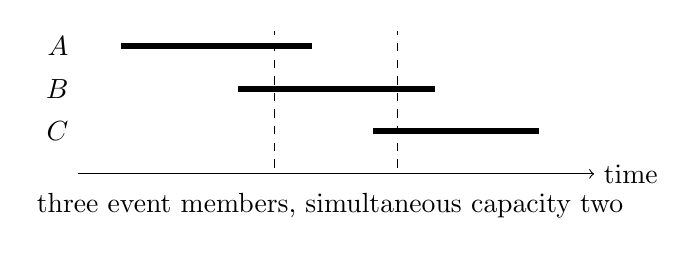
\begin{tikzpicture}[x=0.78cm,y=0.54cm]
\draw[->] (0,0) -- (8.4,0) node[right]{time};
\foreach \y/\lab in {3/A,2/B,1/C}{
  \node[left] at (0,\y) {$\lab$};
}
\draw[line width=2.2pt] (0.7,3) -- (3.8,3);
\draw[line width=2.2pt] (2.6,2) -- (5.8,2);
\draw[line width=2.2pt] (4.8,1) -- (7.5,1);
\draw[dashed] (3.2,0.15) -- (3.2,3.35);
\draw[dashed] (5.2,0.15) -- (5.2,3.35);
\node[align=center] at (4.1,-0.75) {three event members, simultaneous capacity two};
\end{tikzpicture}
\caption{A feasible fixed-time event can be an overlap chain. This differs
from both a clique and the two-member restriction $K=2$.}
\Description{Three intervals form a positive-overlap chain, with at most two
active simultaneously.}
\label{fig:chain}
\end{figure}
